\section{My favourite gadgets}
This is the era of technology. In this era we use different types of devices such as smart phones, computers, pad, telephones, walkie-talkie etc. We can not move a step without the devices. We can communicate with one another using the devices through online or offline. The  devices we see now do not come in a day. The world is now in our hand. We can see or know what is happening in other countries in a moment. In past it was impossible. In figure~\ref{fig:fig2} and figure~\ref{fig:fig3}, I have shown a digital computer and smart phone respectively.
\begin{figure}[h]
    \centering
    \begin{minipage}[b]{.49\textwidth}
    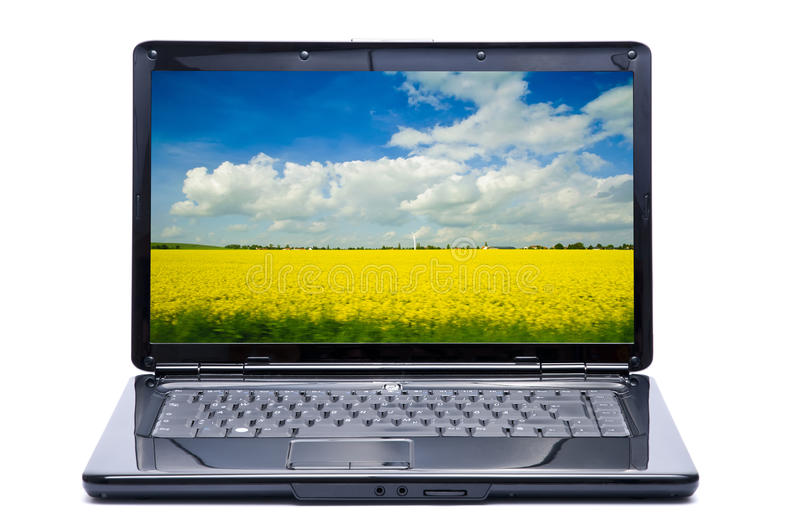
\includegraphics[width = 1\linewidth]{pic/laptop.jpg}
     \caption{Digital Computer} 
     \label{fig:fig2}
    \end{minipage}
    % hfh
    \begin{minipage}[b]{.48\textwidth}
    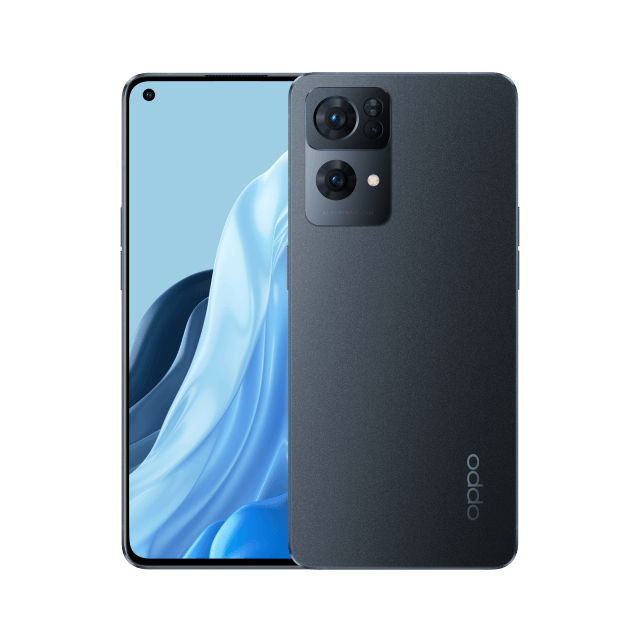
\includegraphics[width = 1\linewidth]{pic/smart_phone.png}
     \caption{Smart Phone} 
     \label{fig:fig3}
    \end{minipage}  
\end{figure}\\
As I am an engineering student of Computer Science and Engineering department, Rajshshahi University, I use many digital devices. I use those devices for academic purposes and personal purposes to communicate with my teachers and others. My favourite gadgets are smart phone and computer. I use these devices very well for my works. Without the devices I can not move at all. Because I am a computer science student. I need this devices to complete my academic study.  For example, when I do programming contest then I must need a personal computer for solving problems as well as availability of internet. If I want to make a calculator using object oriented programming languages, then I need a computer for coding. Smart phone is also needed to contact with others and it is also used for camera feature. The phone with best camera feature is most demanful in market.\\
My favourite gadgets are used to complete our daily activities. As I am a student I am using these devices for my educational purposes. I can use the devices for solving mathematical problem. Such as I can consider equation~\ref{eq : eq1} and equation~\ref{eq : eq2}.
\begin{equation}
    a_1x + b_1y = c_1
    \label{eq : eq1}
\end{equation}
\begin{equation}
    a_2x + b_2y = c_2
    \label{eq : eq2}
\end{equation}
Now I can easily solve the equation using the devices. We just need the parameters of the equations. We can also solve many complex mathematical problems such as differentiation, integration, trigonometric and others. 
We can use many daily needed applications and solve our daily problems. Such applications are Data Base Management System, Spread Sheet which are very essential application for offices, companies and personal tasks. To make a public exam result we must need spreed sheet which help us to complete the work properly. So for using these applications we must need a smart phone or a computer.